% figure-dual-balls-union-intersection.tex
% Dual ball identities: open ball as union of closed, closed as intersection of open
% Requires:
%   \usepackage{tikz}
%   \usetikzlibrary{arrows.meta,positioning,calc}

\begin{center}
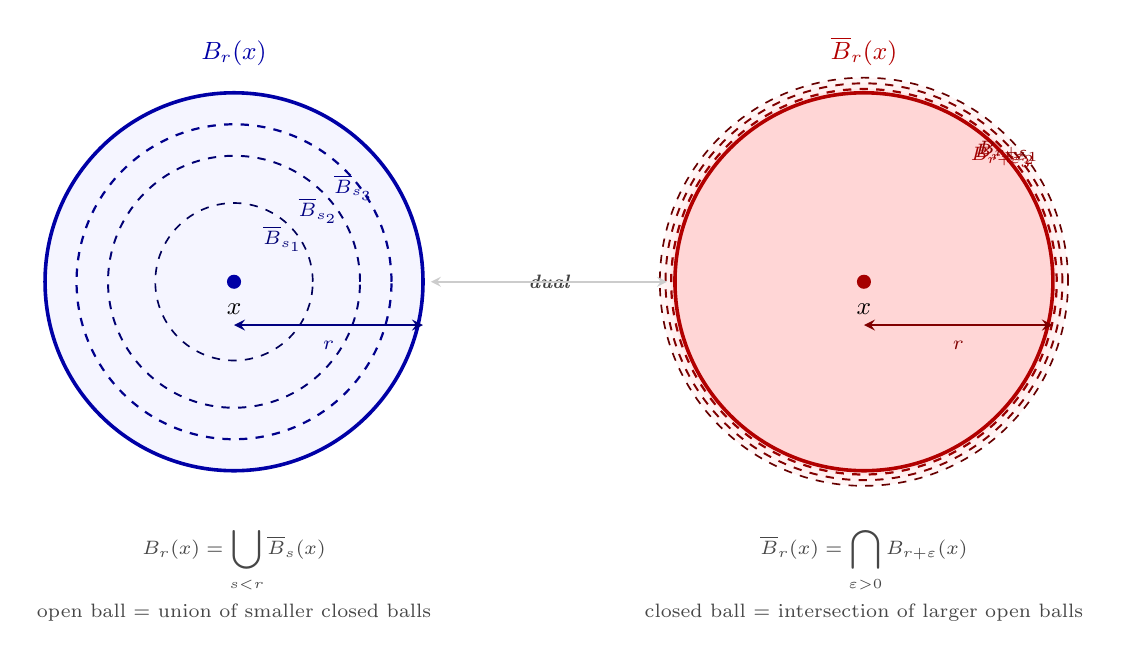
\begin{tikzpicture}[
  dot/.style={circle,fill,inner sep=1.8pt},
  >=stealth,
  lbl/.style={font=\small},
  slbl/.style={font=\scriptsize},
]

% ===== LEFT PANEL: B_r(x) = union of closed balls ================================
\begin{scope}[xshift=-4.0cm]

\def\R{2.4}

% Shaded closed balls at s=0.8, 1.4, 1.9 (building up the open ball)
\fill[blue!14] (0,0) circle (1.9);
\fill[blue!9]  (0,0) circle (2.15);
% The open ball itself
\fill[blue!4]  (0,0) circle (\R);

% Draw closed balls at three radii (dashed)
\draw[blue!35!black, line width=0.6pt, dashed] (0,0) circle (1.0);
\draw[blue!45!black, line width=0.7pt, dashed] (0,0) circle (1.6);
\draw[blue!55!black, line width=0.8pt, dashed] (0,0) circle (2.0);

% Outer open ball boundary (solid)
\draw[blue!65!black, line width=1.3pt] (0,0) circle (\R);

% Center
\node[dot, fill=blue!65!black] at (0,0) {};
\node[lbl, anchor=north] at (0,-0.16) {$x$};

% Radius r arrow
\draw[blue!50!black, <->, line width=0.75pt]
  (0,-0.55) -- ({\R},{ -0.55})
  node[midway, below, slbl, yshift=-2pt] {$r$};

% Closing ball labels
\node[slbl, text=blue!45!black] at (0.62, 0.55) {$\overline{B}_{s_1}$};
\node[slbl, text=blue!50!black] at (1.07, 0.90) {$\overline{B}_{s_2}$};
\node[slbl, text=blue!55!black] at (1.52, 1.20) {$\overline{B}_{s_3}$};

% Title
\node[lbl, text=blue!65!black, font=\small\itshape, anchor=south]
  at (0, {\R+0.22}) {$B_r(x)$};

\end{scope}

% ===== RIGHT PANEL: B̄_r(x) = intersection of open balls ========================
\begin{scope}[xshift=4.0cm]

\def\R{2.4}

% Draw open balls at three radii (dashed, getting smaller toward r)
\fill[red!4]  (0,0) circle ({1.08*\R});
\fill[red!6]  (0,0) circle ({1.05*\R});
\fill[red!10] (0,0) circle ({1.02*\R});

% Closed ball interior (solid fill)
\fill[red!16] (0,0) circle (\R);

% Open ball boundaries
\draw[red!40!black, line width=0.6pt, dashed] (0,0) circle ({1.08*\R});
\draw[red!50!black, line width=0.7pt, dashed] (0,0) circle ({1.05*\R});
\draw[red!60!black, line width=0.8pt, dashed] (0,0) circle ({1.02*\R});

% Closed ball boundary (solid)
\draw[red!70!black, line width=1.3pt] (0,0) circle (\R);

% Center
\node[dot, fill=red!65!black] at (0,0) {};
\node[lbl, anchor=north] at (0,-0.16) {$x$};

% Radius r arrow
\draw[red!50!black, <->, line width=0.75pt]
  (0,-0.55) -- ({\R},{-0.55})
  node[midway, below, slbl, yshift=-2pt] {$r$};

% Open ball labels at offsets
\node[slbl, text=red!55!black] at ({1.065*\R*0.72}, {1.065*\R*0.65}) {$B_{r+\varepsilon_1}$};
\node[slbl, text=red!60!black] at ({1.038*\R*0.72}, {1.038*\R*0.65}) {$B_{r+\varepsilon_2}$};
\node[slbl, text=red!65!black] at ({1.012*\R*0.72}, {1.012*\R*0.65}) {$B_{r+\varepsilon_3}$};

% Closed ball label
\node[lbl, text=red!70!black, font=\small\itshape, anchor=south]
  at (0,{\R+0.22}) {$\overline{B}_r(x)$};

\end{scope}

% ===== Central label ===========================================================
\node[slbl, text=gray!50!black, font=\scriptsize\itshape]
  at (0, 0) {\textbf{dual}};
\draw[gray!40, <->, line width=0.6pt] (-1.5, 0) -- (1.5, 0);

% ===== Captions below both panels (in outer scope, fixed y) ====================
\node[slbl, text=gray!55!black, anchor=north, align=center]
  at (-4.0, -3.0) {$B_r(x)=\displaystyle\bigcup_{s<r}\overline{B}_s(x)$\\[3pt]
                   open ball = union of smaller closed balls};
\node[slbl, text=gray!55!black, anchor=north, align=center]
  at ( 4.0, -3.0) {$\overline{B}_r(x)=\displaystyle\bigcap_{\varepsilon>0}B_{r+\varepsilon}(x)$\\[3pt]
                   closed ball = intersection of larger open balls};

\end{tikzpicture}
\end{center}